
%% bare_jrnl.tex
%% V1.4
%% 2012/12/27
%% by Michael Shell
%% see http://www.michaelshell.org/
%% for current contact information.
%%
%% This is a skeleton file demonstrating the use of IEEEtran.cls
%% (requires IEEEtran.cls version 1.8 or later) with an IEEE journal paper.
%%
%% Support sites:
%% http://www.michaelshell.org/tex/ieeetran/
%% http://www.ctan.org/tex-archive/macros/latex/contrib/IEEEtran/
%% and
%% http://www.ieee.org/



% *** Authors should verify (and, if needed, correct) their LaTeX system  ***
% *** with the testflow diagnostic prior to trusting their LaTeX platform ***
% *** with production work. IEEE's font choices can trigger bugs that do  ***
% *** not appear when using other class files.                            ***
% The testflow support page is at:
% http://www.michaelshell.org/tex/testflow/


%%*************************************************************************
%% Legal Notice:
%% This code is offered as-is without any warranty either expressed or
%% implied; without even the implied warranty of MERCHANTABILITY or
%% FITNESS FOR A PARTICULAR PURPOSE! 
%% User assumes all risk.
%% In no event shall IEEE or any contributor to this code be liable for
%% any damages or losses, including, but not limited to, incidental,
%% consequential, or any other damages, resulting from the use or misuse
%% of any information contained here.
%%
%% All comments are the opinions of their respective authors and are not
%% necessarily endorsed by the IEEE.
%%
%% This work is distributed under the LaTeX Project Public License (LPPL)
%% ( http://www.latex-project.org/ ) version 1.3, and may be freely used,
%% distributed and modified. A copy of the LPPL, version 1.3, is included
%% in the base LaTeX documentation of all distributions of LaTeX released
%% 2003/12/01 or later.
%% Retain all contribution notices and credits.
%% ** Modified files should be clearly indicated as such, including  **
%% ** renaming them and changing author support contact information. **
%%
%% File list of work: IEEEtran.cls, IEEEtran_HOWTO.pdf, bare_adv.tex,
%%                    bare_conf.tex, bare_jrnl.tex, bare_jrnl_compsoc.tex,
%%                    bare_jrnl_transmag.tex
%%*************************************************************************

% Note that the a4paper option is mainly intended so that authors in
% countries using A4 can easily print to A4 and see how their papers will
% look in print - the typesetting of the document will not typically be
% affected with changes in paper size (but the bottom and side margins will).
% Use the testflow package mentioned above to verify correct handling of
% both paper sizes by the user's LaTeX system.
%
% Also note that the "draftcls" or "draftclsnofoot", not "draft", option
% should be used if it is desired that the figures are to be displayed in
% draft mode.
%
\documentclass[journal,twocolumns]{IEEEtran}
%
% If IEEEtran.cls has not been installed into the LaTeX system files,
% manually specify the path to it like:
% \documentclass[journal]{../sty/IEEEtran}





% Some very useful LaTeX packages include:
% (uncomment the ones you want to load)


% *** MISC UTILITY PACKAGES ***
%
%\usepackage{ifpdf}
% Heiko Oberdiek's ifpdf.sty is very useful if you need conditional
% compilation based on whether the output is pdf or dvi.
% usage:
% \ifpdf
%   % pdf code
% \else
%   % dvi code
% \fi
% The latest version of ifpdf.sty can be obtained from:
% http://www.ctan.org/tex-archive/macros/latex/contrib/oberdiek/
% Also, note that IEEEtran.cls V1.7 and later provides a builtin
% \ifCLASSINFOpdf conditional that works the same way.
% When switching from latex to pdflatex and vice-versa, the compiler may
% have to be run twice to clear warning/error messages.






% *** CITATION PACKAGES ***
%
%\usepackage{cite}
% cite.sty was written by Donald Arseneau
% V1.6 and later of IEEEtran pre-defines the format of the cite.sty package
% \cite{} output to follow that of IEEE. Loading the cite package will
% result in citation numbers being automatically sorted and properly
% "compressed/ranged". e.g., [1], [9], [2], [7], [5], [6] without using
% cite.sty will become [1], [2], [5]--[7], [9] using cite.sty. cite.sty's
% \cite will automatically add leading space, if needed. Use cite.sty's
% noadjust option (cite.sty V3.8 and later) if you want to turn this off
% such as if a citation ever needs to be enclosed in parenthesis.
% cite.sty is already installed on most LaTeX systems. Be sure and use
% version 4.0 (2003-05-27) and later if using hyperref.sty. cite.sty does
% not currently provide for hyperlinked citations.
% The latest version can be obtained at:
% http://www.ctan.org/tex-archive/macros/latex/contrib/cite/
% The documentation is contained in the cite.sty file itself.






% *** GRAPHICS RELATED PACKAGES ***
%
\ifCLASSINFOpdf
\usepackage[pdftex]{graphicx}
  % declare the path(s) where your graphic files are
  %\graphicspath{{../pdf/}{../jpeg/}}
  % and their extensions so you won't have to specify these with
  % every instance of \includegraphics
  % \DeclareGraphicsExtensions{.pdf,.jpeg,.png}
\else
  % or other class option (dvipsone, dvipdf, if not using dvips). graphicx
  % will default to the driver specified in the system graphics.cfg if no
  % driver is specified.
  % \usepackage[dvips]{graphicx}
  % declare the path(s) where your graphic files are
  % \graphicspath{{../eps/}}
  % and their extensions so you won't have to specify these with
  % every instance of \includegraphics
  % \DeclareGraphicsExtensions{.eps}
\fi
% graphicx was written by David Carlisle and Sebastian Rahtz. It is
% required if you want graphics, photos, etc. graphicx.sty is already
% installed on most LaTeX systems. The latest version and documentation
% can be obtained at: 
% http://www.ctan.org/tex-archive/macros/latex/required/graphics/
% Another good source of documentation is "Using Imported Graphics in
% LaTeX2e" by Keith Reckdahl which can be found at:
% http://www.ctan.org/tex-archive/info/epslatex/
%
% latex, and pdflatex in dvi mode, support graphics in encapsulated
% postscript (.eps) format. pdflatex in pdf mode supports graphics
% in .pdf, .jpeg, .png and .mps (metapost) formats. Users should ensure
% that all non-photo figures use a vector format (.eps, .pdf, .mps) and
% not a bitmapped formats (.jpeg, .png). IEEE frowns on bitmapped formats
% which can result in "jaggedy"/blurry rendering of lines and letters as
% well as large increases in file sizes.
%
% You can find documentation about the pdfTeX application at:
% http://www.tug.org/applications/pdftex


% Prof. Forbes math packages
\usepackage{amsmath} % cmex10
\usepackage{amssymb}
\usepackage{amsthm}
\usepackage{bm}
\usepackage{mathrsfs}
\usepackage{wrapfig}

%accents
\usepackage[latin1]{inputenc} 

% *** MATH PACKAGES ***
%
% \usepackage[cmex10]{amsmath}
% A popular package from the American Mathematical Society that provides
% many useful and powerful commands for dealing with mathematics. If using
% it, be sure to load this package with the cmex10 option to ensure that
% only type 1 fonts will utilized at all point sizes. Without this option,
% it is possible that some math symbols, particularly those within
% footnotes, will be rendered in bitmap form which will result in a
% document that can not be IEEE Xplore compliant!
%
% Also, note that the amsmath package sets \interdisplaylinepenalty to 10000
% thus preventing page breaks from occurring within multiline equations. Use:
%\interdisplaylinepenalty=2500
% after loading amsmath to restore such page breaks as IEEEtran.cls normally
% does. amsmath.sty is already installed on most LaTeX systems. The latest
% version and documentation can be obtained at:
% http://www.ctan.org/tex-archive/macros/latex/required/amslatex/math/





% *** SPECIALIZED LIST PACKAGES ***
%
%\usepackage{algorithmic}
% algorithmic.sty was written by Peter Williams and Rogerio Brito.
% This package provides an algorithmic environment fo describing algorithms.
% You can use the algorithmic environment in-text or within a figure
% environment to provide for a floating algorithm. Do NOT use the algorithm
% floating environment provided by algorithm.sty (by the same authors) or
% algorithm2e.sty (by Christophe Fiorio) as IEEE does not use dedicated
% algorithm float types and packages that provide these will not provide
% correct IEEE style captions. The latest version and documentation of
% algorithmic.sty can be obtained at:
% http://www.ctan.org/tex-archive/macros/latex/contrib/algorithms/
% There is also a support site at:
% http://algorithms.berlios.de/index.html
% Also of interest may be the (relatively newer and more customizable)
% algorithmicx.sty package by Szasz Janos:
% http://www.ctan.org/tex-archive/macros/latex/contrib/algorithmicx/




% *** ALIGNMENT PACKAGES ***
%
%\usepackage{array}
% Frank Mittelbach's and David Carlisle's array.sty patches and improves
% the standard LaTeX2e array and tabular environments to provide better
% appearance and additional user controls. As the default LaTeX2e table
% generation code is lacking to the point of almost being broken with
% respect to the quality of the end results, all users are strongly
% advised to use an enhanced (at the very least that provided by array.sty)
% set of table tools. array.sty is already installed on most systems. The
% latest version and documentation can be obtained at:
% http://www.ctan.org/tex-archive/macros/latex/required/tools/


% IEEEtran contains the IEEEeqnarray family of commands that can be used to
% generate multiline equations as well as matrices, tables, etc., of high
% quality.




% *** SUBFIGURE PACKAGES ***
%\ifCLASSOPTIONcompsoc
%  \usepackage[caption=false,font=normalsize,labelfont=sf,textfont=sf]{subfig}
%\else
%  \usepackage[caption=false,font=footnotesize]{subfig}
%\fi
% subfig.sty, written by Steven Douglas Cochran, is the modern replacement
% for subfigure.sty, the latter of which is no longer maintained and is
% incompatible with some LaTeX packages including fixltx2e. However,
% subfig.sty requires and automatically loads Axel Sommerfeldt's caption.sty
% which will override IEEEtran.cls' handling of captions and this will result
% in non-IEEE style figure/table captions. To prevent this problem, be sure
% and invoke subfig.sty's "caption=false" package option (available since
% subfig.sty version 1.3, 2005/06/28) as this is will preserve IEEEtran.cls
% handling of captions.
% Note that the Computer Society format requires a larger sans serif font
% than the serif footnote size font used in traditional IEEE formatting
% and thus the need to invoke different subfig.sty package options depending
% on whether compsoc mode has been enabled.
%
% The latest version and documentation of subfig.sty can be obtained at:
% http://www.ctan.org/tex-archive/macros/latex/contrib/subfig/




% *** FLOAT PACKAGES ***
%
%\usepackage{fixltx2e}
% fixltx2e, the successor to the earlier fix2col.sty, was written by
% Frank Mittelbach and David Carlisle. This package corrects a few problems
% in the LaTeX2e kernel, the most notable of which is that in current
% LaTeX2e releases, the ordering of single and double column floats is not
% guaranteed to be preserved. Thus, an unpatched LaTeX2e can allow a
% single column figure to be placed prior to an earlier double column
% figure. The latest version and documentation can be found at:
% http://www.ctan.org/tex-archive/macros/latex/base/


%\usepackage{stfloats}
% stfloats.sty was written by Sigitas Tolusis. This package gives LaTeX2e
% the ability to do double column floats at the bottom of the page as well
% as the top. (e.g., "\begin{figure*}[!b]" is not normally possible in
% LaTeX2e). It also provides a command:
%\fnbelowfloat
% to enable the placement of footnotes below bottom floats (the standard
% LaTeX2e kernel puts them above bottom floats). This is an invasive package
% which rewrites many portions of the LaTeX2e float routines. It may not work
% with other packages that modify the LaTeX2e float routines. The latest
% version and documentation can be obtained at:
% http://www.ctan.org/tex-archive/macros/latex/contrib/sttools/
% Do not use the stfloats baselinefloat ability as IEEE does not allow
% \baselineskip to stretch. Authors submitting work to the IEEE should note
% that IEEE rarely uses double column equations and that authors should try
% to avoid such use. Do not be tempted to use the cuted.sty or midfloat.sty
% packages (also by Sigitas Tolusis) as IEEE does not format its papers in
% such ways.
% Do not attempt to use stfloats with fixltx2e as they are incompatible.
% Instead, use Morten Hogholm'a dblfloatfix which combines the features
% of both fixltx2e and stfloats:
%
% \usepackage{dblfloatfix}
% The latest version can be found at:
% http://www.ctan.org/tex-archive/macros/latex/contrib/dblfloatfix/




%\ifCLASSOPTIONcaptionsoff
%  \usepackage[nomarkers]{endfloat}
% \let\MYoriglatexcaption\caption
% \renewcommand{\caption}[2][\relax]{\MYoriglatexcaption[#2]{#2}}
%\fi
% endfloat.sty was written by James Darrell McCauley, Jeff Goldberg and 
% Axel Sommerfeldt. This package may be useful when used in conjunction with 
% IEEEtran.cls'  captionsoff option. Some IEEE journals/societies require that
% submissions have lists of figures/tables at the end of the paper and that
% figures/tables without any captions are placed on a page by themselves at
% the end of the document. If needed, the draftcls IEEEtran class option or
% \CLASSINPUTbaselinestretch interface can be used to increase the line
% spacing as well. Be sure and use the nomarkers option of endfloat to
% prevent endfloat from "marking" where the figures would have been placed
% in the text. The two hack lines of code above are a slight modification of
% that suggested by in the endfloat docs (section 8.4.1) to ensure that
% the full captions always appear in the list of figures/tables - even if
% the user used the short optional argument of \caption[]{}.
% IEEE papers do not typically make use of \caption[]'s optional argument,
% so this should not be an issue. A similar trick can be used to disable
% captions of packages such as subfig.sty that lack options to turn off
% the subcaptions:
% For subfig.sty:
% \let\MYorigsubfloat\subfloat
% \renewcommand{\subfloat}[2][\relax]{\MYorigsubfloat[]{#2}}
% However, the above trick will not work if both optional arguments of
% the \subfloat command are used. Furthermore, there needs to be a
% description of each subfigure *somewhere* and endfloat does not add
% subfigure captions to its list of figures. Thus, the best approach is to
% avoid the use of subfigure captions (many IEEE journals avoid them anyway)
% and instead reference/explain all the subfigures within the main caption.
% The latest version of endfloat.sty and its documentation can obtained at:
% http://www.ctan.org/tex-archive/macros/latex/contrib/endfloat/
%
% The IEEEtran \ifCLASSOPTIONcaptionsoff conditional can also be used
% later in the document, say, to conditionally put the References on a 
% page by themselves.




% *** PDF, URL AND HYPERLINK PACKAGES ***
%
%\usepackage{url}
% url.sty was written by Donald Arseneau. It provides better support for
% handling and breaking URLs. url.sty is already installed on most LaTeX
% systems. The latest version and documentation can be obtained at:
% http://www.ctan.org/tex-archive/macros/latex/contrib/url/
% Basically, \url{my_url_here}.




% *** Do not adjust lengths that control margins, column widths, etc. ***
% *** Do not use packages that alter fonts (such as pslatex).         ***
% There should be no need to do such things with IEEEtran.cls V1.6 and later.
% (Unless specifically asked to do so by the journal or conference you plan
% to submit to, of course. )


% correct bad hyphenation here
% \hyphenation{op-tical net-works semi-conduc-tor}
\hyphenation{La-grange La-grang-ian dy-nam-ics}

% Prof. Forbes' custom commands here! Some of these commands are from Chris Damaren, Gabe D'Eleuterio, Tim Barfoot, Paul Furgal, Adam Philip. Thanks to all!

% Matrix command
\newcommand{\bma}[1]{\left[\begin{array}{#1}}
\newcommand{\ema}{\end{array}\right]}
\newcommand{\trans}{{\ensuremath{\mathsf{T}}}} % transpose
\newcommand{\utimes}{ {\raisebox{-0.6ex}{ \kern-1.0ex\raisebox{0.6ex}{ \small $\mathsf{v}$}}} } % 
\newcommand{\onehalf}{\mbox{$\textstyle{\frac{1}{2}}$}}

% Bold symbols
\DeclareMathAlphabet{\mbf}{OT1}{ptm}{b}{n} % for bold face Roman
\newcommand{\mbs}[1]{{\boldsymbol{#1}}} % for bold face Greek

% Other bold symbols 
\newcommand{\mbfbar}[1]{{\bar{\mbf{#1}}}}
\newcommand{\mbfhat}[1]{{\hat{\mbf{#1}}}}
\newcommand{\mbftilde}[1]{{\tilde{\mbf{#1}}}}
\newcommand{\mbsbar}[1]{{\bar{\boldsymbol{#1}}}}
\newcommand{\mbshat}[1]{{\hat{\boldsymbol{#1}}}}
\newcommand{\mbstilde}[1]{{\tilde{\boldsymbol{#1}}}}

% Physical Space, physical vectors, a vectrix, etc. 
\newcommand{\pspace}{\mathbb{P}} 
\newcommand{\ura}[1]{{\underrightarrow{{#1}}}}
\newcommand{\vectrix}[1]{\ensuremath \underrightarrow{\boldsymbol{\mathcal{F}}}_{#1}}
\def\fdota{{\raisebox{-2pt}{\LARGE $\cdot$}}}
\def\fdotb{{\raisebox{-0.6ex}{ \kern0.2ex\raisebox{0.8ex}{\tiny $\hspace*{-1ex}\circ$}}}}
\def\fddota{{\raisebox{-2pt}{\LARGE $\cdot\hspace*{-0.2ex}\cdot$}}}
\def\fddotb{{\raisebox{-0.6ex}{ \kern0.2ex\raisebox{0.8ex}{\tiny $\hspace*{-1ex}\circ\circ$}}}}
\newcommand{\fdot}[1]{{^{\fdota{\mbox{\footnotesize${#1}$}}}}}
\newcommand{\fddot}[1]{{^{\fddota{\mbox{\footnotesize${#1}$}}}}}


% Short form for equations
\newcommand{\beq}{\begin{equation}}
\newcommand{\eeq}{\end{equation}}
\newcommand{\bdis}{\begin{displaymath}}
\newcommand{\edis}{\end{displaymath}}
\newcommand{\beqarray}{\begin{eqnarray}}
\newcommand{\eeqarray}{\end{eqnarray}}
\newcommand{\beqarraynn}{\begin{eqnarray*}}
\newcommand{\eeqarraynn}{\end{eqnarray*}}

%Must be equal to ...
\newcommand{\mbeq}{\overset{!}{=}}

% Matrices shortcut
\newcommand{\crossop}[3]{\bma{ccc} 0 & -#3 & #2 \\ #3 & 0 & -#1 \\ -#2 & #1 & 0 \ema}
\newcommand{\matr}[9]{\bma{ccc} #1 & #2 & #3 \\ #4 & #5 & #6 \\ #7 & #8 & #9 \ema}
\newcommand{\colvec}[3]{\bma{c} #1 \\ #2 \\ #3 \ema}
\newcommand{\rowvec}[3]{\bma{ccc} #1 & #2 & #3 \ema}
\newcommand{\Cone}[1]{\matr{1}{0}{0}{0}{\cos(#1)}{\sin(#1)}{0}{-\sin(#1)}{\cos(#1)}}
\newcommand{\Ctwo}[1]{\matr{\cos(#1)}{0}{-\sin(#1)}{0}{1}{0}{\sin(#1)}{0}{\cos(#1)}}
\newcommand{\Cthree}[1]{\matr{\cos(#1)}{\sin(#1)}{0}{-\sin(#1)}{\cos(#1)}{0}{0}{0}{1}}


\begin{document}

\title{Project Kinematics - ADR Spacecraft}


\author{Fr�d�ric Berdoz, 260867318}% <-this % stops a space
\markboth{MECH 642 -- Advanced Dynamics}%
{Advanced Dynamics}

\maketitle

\IEEEpeerreviewmaketitle

\section{Geometrical parametrization}
\IEEEPARstart{I}{n} order to perform an accurate kinematic analysis on the spacecraft and the debris, it is necessary to describe fully and accurately their geometry with parameters.  Let $o$ be a fixed point on earth. The spacecraft is modeled as a closed end hollow cylinder with a wall thickness $t_s$, an outer radius $\rho_o$ and a length $l_s$. Its main propeller P1 is attached to the main body at the point $p$, at the center of its base. On the top, the two auxiliary propellers P2 and P3 sit diametrically opposite each other, at a distance $\rho_p$ from $A_s$ (the spacecraft axis). The two reaction wheels W1 and W2 are modeled as full cylinders of radius and length $\rho_1$ and $l_1$ (respectively $\rho_2$ and $l_2$). W1 is oriented radially and W2 axially, in such a way that their center of gravity $g_{1}$ and $g_{2}$ are both on $A_s$. Moreover, W1 is aligned with P2 and P3. The length of point $g_{1}$ (and $g_{2}$) relative to point $p$ is $z_1$ (respectively $z_2$). The centre of mass of the wall $g_s$ coincide with the geometrical centre of the spacecraft. With this symmetrical geometry, the spacecraft centre of gravity $g$ must lie on the main axis $A_s$. Let $z_g$ be the length of $g$ relative to $p$ and let $m_{s}$, $m_{1}$ and $m_{2}$ be the mass of the spacecraft wall, of W1 and of W2, respectively. Neglecting the mass of all the other parts, it yields
\beq
z_g=\frac{\frac{l_s}{2}m_s+z_1m_1+z_2m_2}{m_{w}+m_1+m_2}.
\label{eq:zs}
\eeq
To simplify, the debris is modeled as a full cube of size $l_d$. Finally, let the point $w$ be one of its corner and $g_d$ its center of gravity.

\section{Reference frames}
(From this point, the notation used is from \cite{Course}.) In this project, 6 different reference frames will be used:
\begin{itemize}
\item $\mathcal{F}_e$ : An  inertial reference frame attached to the earth.
\item $\mathcal{F}_s$ : The reference frame attached to the body of the spacecraft. $\ura{s}^2$ is aligned with W1, $\ura{s}^3$ is aligned with $A_s$ and oriented towards the front of the spacecraft. Finally, $\ura{s}^1=\ura{s}^2\times\ura{s}^3$.
\item $\mathcal{F}_a$ : The reference frame attached to W1, obtained by rotating $\mathcal{F}_s$  about $\ura{s}^2=\ura{a}^2$. The angle of this rotation is refered to as $\alpha$.
\item $\mathcal{F}_b$ : The reference frame attached to W2, obtained by rotating $\mathcal{F}_s$  about $\ura{s}^3=\ura{b}^3$. The angle of this rotation is refered to as $\beta$.
\item $\mathcal{F}_d$ : The reference frame attached to the body of the debris and aligned with its edges.
\item $\mathcal{F}_u$ : The inertial reference frame obtained  by rotating $\mathcal{F}_e$ in such a way that$\ura{e}^3$ goes to $\ura{u}^3$, which is itself aligned with $\ura{v}^{g_do/e}$. (This frame is not really useful for the dynamic/kinematic part but might help if some control is added at the end of the project.)
\end{itemize}

\begin{figure}[h]
    \centering
        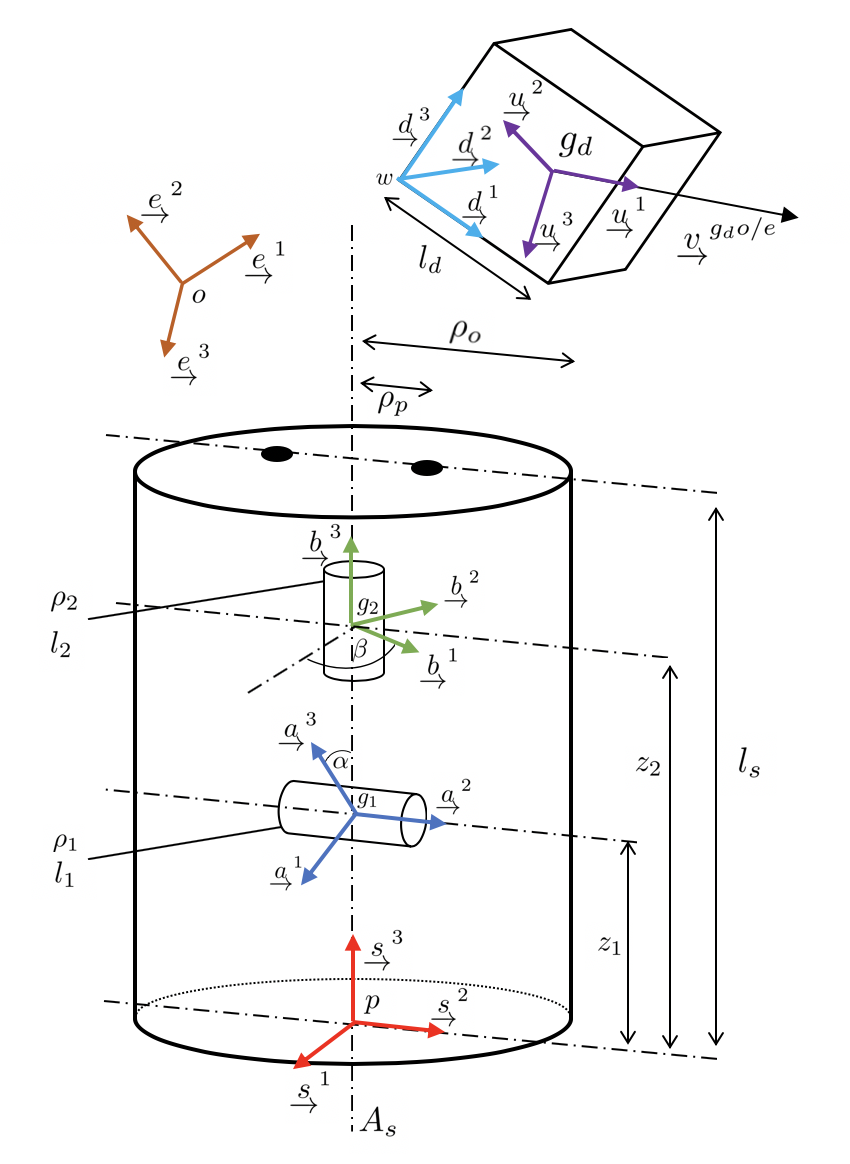
\includegraphics[width=.4\textwidth]{Kinematics_illustration}
    \caption{Geometrical parametrization and reference frames definition.}
    \label{fig:Frames}
\end{figure}


\section{Attitude description}
Since this problem is highly three dimensional, all the mutual configurations of the different reference frames are likely to happen. Using attitude parametrization that are not global or have kinematic singularities is risky and might in the end complicate the problem even more. This is why Direction Cosine Matrices will mostly be used. However, one DCM ($\mbf{C}_{ue}$) will be parametrized using the Angle/Axis (Rodrigues's formula), but it will be constant in time and kinematic singularities will not be a problem.

\section{Measurables}
This problem has 14 degrees of freedom (6 for the shell, 1 for each reaction wheel and 6 for the debris). Therefore, in order to have a well defined and observable problem, 28 independent measurables are needed (14 positions and 14 velocities). The following assumptions will be made:
\begin{itemize}
\item The earth has a radar system that can determine $\mbf{r}_e^{g_do}$, $\mbf{v}^{g_do/e}_e$, $\mbf{r}_e^{po}$ and $\mbf{v}^{po/e}_e$. Moreover, it communicates with the spacecraft sensors in order to determine $\mbf{s}^1_e,\mbf{s}^2_e$ and $\mbf{s}^3_e$. Lastly, it can compute $\mbs{\omega}_e^{se}$.
\item The spacecraft system knows $\alpha$, $\beta$, $\dot{\alpha}$ and $\dot{\beta}$.
\item The spacecraft has sensors that can observe the debris' behavior, i.e. $\mbf{d}^1_s,\mbf{d}^2_s$, $\mbf{d}^3_s$ and $\mbs{\omega}_s^{ds}$  (It is assumed that the radars on earth are too far to observe directly the orientation and the spin of the debris).
\end{itemize}
All the other states can be derived from these 28 variables.

\section{Direction Cosine Matrices}
\textit{A priori}, 15 DCM are needed in order to be able to jump freely between 6 reference frames. However, all of them can be expressed as a combination of 5 elementary DCM (or their transpose). Here is a possible set that can be used to derived all the other DCM:
\begin{align}
\mbf{C}_{es} &=\vectrix{e}\cdot\vectrix{s}^\trans=\rowvec{{\mbf{s}_e^1}}{{\mbf{s}_e^2}}{{\mbf{s}_e^3}}, \label{eq:Ces} \\
\mbf{C}_{as}&=\mbf{C}_2(\alpha)=\Ctwo{\alpha},  \label{eq:Cas}\\
\mbf{C}_{bs}&=\mbf{C}_3(\beta)=\Cthree{\beta},  \label{eq:Cbs}\\
\mbf{C}_{sd}&=\vectrix{s}\cdot\vectrix{d}^\trans=\rowvec{{\mbf{d}_s^1}}{{\mbf{d}_s^2}}{{\mbf{d}_s^3}}  \label{eq:Csd}.
\end{align}
Lastly, the way $\mathcal{F}_{u}$ was previously defined does not determine uniquely $\mbf{C}_{ue}$. Therefore, the following conventions will be used:
\beq
\mbf{C}_{ue}=\cos(\phi_v)\mbf{1}+(1-\cos(\phi_v))\mbf{a}_v\mbf{a}_v^\trans-\sin(\phi_v)\mbf{a}_v^\times
\label{eq:Cue2}
\eeq
where, using $v_d={\vert\vert\mbf{v}_e^{g_do/e}\vert\vert}_2$,
\begin{align*}
\phi_v & =
\left\{ 
\begin{array}{rcl} 
	0 & \mbox{for} & v_d=0 \\
	\arccos\left(\frac{\mbf{1}_3^\trans\mbf{v}_e^{g_do/e}}{v_d}\right) & \mbox{for} & v_d\neq0 \, ,
\end{array}
\right. \\
\mbf{a}_v &=
\left\{
\begin{array}{rcl} 
	\mbf{0} & \mbox{for} & \phi_v\in\{0, \pi\} \\
	\frac{\mbf{1}_3^\times\mbf{v}_e^{g_do/e}}{v_d\sin(\phi_v)} & \mbox{for} & \phi_v\not\in\{0, \pi\} \, .
\end{array} 
\right.
\end{align*}
As discussed in the Proposal, $\ura{v}^{g_do/e}$ is assumed to be constant in time. Therefore, $\mbf{C}_{ue}$ is also constant in time, i.e. $\ura{\omega}^{ue}=\ura{0}$.
\section{Angular Velocities}
As for the DCM, a set of 5 angular velocity physical vectors is sufficient to describe every possible kinematic transformation. In particular,
\begin{align}
\ura{\omega}^{es}&=\vectrix{e}^\trans\mbs{\omega}_e^{es}=-\vectrix{e}^\trans\mbs{\omega}_e^{se},\\
\ura{\omega}^{as}&=\vectrix{s}\mbf{1}_2\dot{\alpha}=\vectrix{a}\mbf{1}_2\dot{\alpha},\\
\ura{\omega}^{bs}&=\vectrix{s}\mbf{1}_3\dot{\beta}=\vectrix{b}\mbf{1}_3\dot{\beta},\\
\ura{\omega}^{sd}&=\vectrix{s}^\trans\mbs{\omega}_s^{sd}=-\vectrix{s}^\trans\mbs{\omega}_s^{ds},\\
\ura{\omega}^{ue}&= \ura{0}.
\end{align}

\section{Components Parametrization}
Due to the cylindrical symmetry of the spacecraft and the reaction wheels, the components of the physical vectors resolved in frame $\mathcal{F}_s$, $\mathcal{F}_a$ and $\mathcal{F}_b$ will be parametrized using the cylindrical coordinates. Let $dm_s$, $dm_1$ and $dm_2$ be material elements of the spacecraft wall, of W1 and of W2, respectively. The parametrization of the components of $\mbf{r}_s^{dm_sp}$, $\mbf{r}_a^{dm_1g_1}$ and $\mbf{r}_b^{dm_2g_2}$ will be done accordingly to Figure \ref{fig:Coordinates}.
\begin{figure}[h]
    \centering
        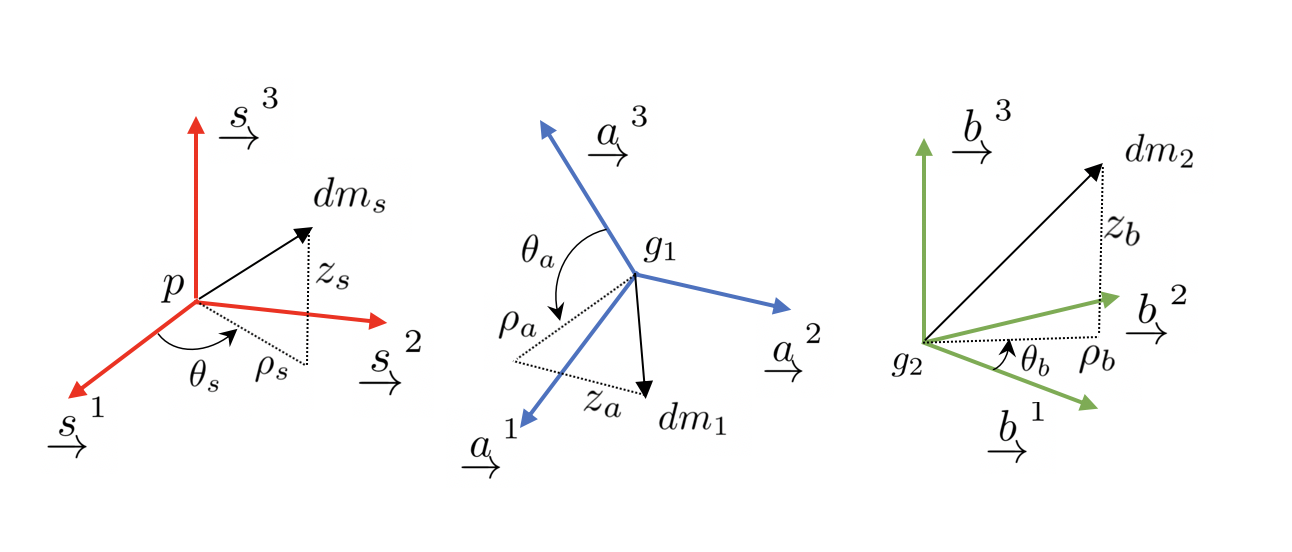
\includegraphics[width=.45\textwidth]{Kinematics_illustration2}
    \caption{Component parametrization in $\mathcal{F}_s$, $\mathcal{F}_a$ and $\mathcal{F}_b$.}
    \label{fig:Coordinates}
\end{figure}

As for the debris, the position of its material elements $dm_d$ relative to $g_d$ resolved in $\mathcal{F}_d$ will be described using a cartesian coordinate system. More precisely, $x_d$, $y_d$ and $z_d$ for the components along $\ura{d}^1$, $\ura{d}^2$ and $\ura{d}^3$, respectively.  In matrix form:
\begin{align*}
\mbf{r}_s^{dm_sp}=\colvec{\rho_s\cos(\theta_s)}{\rho_s\sin(\theta_s)}{z_s}, \quad & \mbf{r}_a^{dm_1g_1}=\colvec{\rho_a\cos(\theta_a)}{z_a}{\rho_a\sin(\theta_a)}, \\
\mbf{r}_b^{dm_2g_2}=\colvec{\rho_b\cos(\theta_b)}{\rho_b\sin(\theta_b)}{z_b}, \quad &  \mbf{r}_d^{dm_dg_d}=\colvec{x_d}{y_d}{z_d}.
\label{eq:components}
\end{align*}

All the mathematical tools are now derived in order to express the position, velocity and acceleration of any material element in the inertial reference frame $\mathcal{F}_e$ and in function of the measurables.

\section{Position}
\begin{align}
\ura{r}^{dm_so} & = \vectrix{e}^\trans\left(\mbf{r}_e^{po}+\mbf{C}_{es}\mbf{r}_s^{dm_sp}\right), \\
\ura{r}^{dm_1o} & = \vectrix{e}^\trans\left(\mbf{r}_e^{po}+\mbf{C}_{es}\mbf{1}_3z_1+\mbf{C}_{es}\mbf{C}_{as}^\trans\mbf{r}_a^{dm_1g_1}\right), \\
\ura{r}^{dm_2o} & = \vectrix{e}^\trans\left(\mbf{r}_e^{po}+\mbf{C}_{es}\mbf{1}_3z_2+\mbf{C}_{es}\mbf{C}_{bs}^\trans\mbf{r}_b^{dm_2g_2}\right), \\
\ura{r}^{dm_do} & = \vectrix{e}^\trans\left(\mbf{r}_e^{g_do}+\mbf{C}_{es}\mbf{C}_{sd}\mbf{r}_d^{dm_dg_d}\right).
\end{align}

\section{Velocity}
\begin{align}
\ura{v}^{dm_so/e} & = \vectrix{e}^\trans\left(\mbf{v}_e^{po/e}+{\mbs{\omega}_{e}^{se}}^\times\mbf{C}_{es}\mbf{r}_s^{dm_sp}\right), 
\\ 
\ura{v}^{dm_1o/e} & = \vectrix{e}^\trans\left(\left[\mbf{C}_{es}\mbf{1}_2\dot{\alpha}+\mbs{\omega}_e^{se}\right]^\times\mbf{C}_{es}\mbf{C}_{as}^\trans\mbf{r}_a^{dm_1g_1}\right. 
\nonumber \\ & \quad \left. +\, {\mbs{\omega}_e^{se}}^\times\mbf{C}_{es}\mbf{1}_3z_1+\mbf{v}_e^{po/e} \right), 
\\ 
\ura{v}^{dm_2o/e} & = \vectrix{e}^\trans\left(\left[\mbf{C}_{es}\mbf{1}_3\dot{\beta}+\mbs{\omega}_e^{se}\right]^\times\mbf{C}_{es}\mbf{C}_{bs}^\trans\mbf{r}_b^{dm_2g_2}\right. 
\nonumber \\ & \quad \left. +\, {\mbs{\omega}_e^{se}}^\times\mbf{C}_{es}\mbf{1}_3z_2+\mbf{v}_e^{po/e} \right), 
\\ \ura{v}^{dm_do/e} & = \vectrix{e}^\trans\left( \left[\mbf{C}_{es}\mbs{\omega}_s^{ds}+\mbs{\omega}_e^{se}\right]^\times\mbf{C}_{es}\mbf{C}_{sd}\mbf{r}_d^{dm_dg_d}\right.
\nonumber\\ & \quad \left.+\mbf{v}_e^{g_do/e}\right).
\end{align}

\section{Acceleration}
\begin{align}
\ura{a}^{dm_so/e} & = \vectrix{e}^\trans\left(
\dot{\mbf{v}}_e^{po/e}+\left.\dot{\mbs{\omega}}_e^{se}\right.^\times\mbf{C}_{es}\mbf{r}_s^{dm_sp}
\right. \nonumber \\ & \quad \left.
+\,{\mbs{\omega}_e^{se}}^\times{\mbs{\omega}_e^{se}}^\times\,\mbf{C}_{es}\mbf{r}_s^{dm_sp}
\right), 
\\
\ura{a}^{dm_1o/e} & = \vectrix{e}^\trans\left(
\left[\mbf{C}_{es}\mbf{1}_2\ddot{\alpha}+\dot{\mbs{\omega}}_e^{se}
-\mbf{C}_{es}(\mbf{1}_2\dot{\alpha})^\times\mbs{\omega}_e^{se}\right]^\times \dots
\right. \nonumber \\ & \quad \left.
\mbf{C}_{es}\mbf{C}_{as}^\trans\mbf{r}_a^{dm_1g_1}
+\left[\mbf{C}_{es}\mbf{1}_2\dot{\alpha}+\mbs{\omega}_e^{se}\right]^\times \dots
\right. \nonumber \\ & \quad \left.
\left[\mbf{C}_{es}\mbf{1}_2\dot{\alpha}+\mbs{\omega}_e^{se}\right]^\times\mbf{C}_{es}\mbf{C}_{as}^\trans\mbf{r}_a^{dm_1g_1}
\right. \nonumber \\ & \quad \left.
+\left[\left.\dot{\mbs{\omega}}_e^{se}\right.^\times+{\mbs{\omega}_e^{se}}^\times{\mbs{\omega}_e^{se}}^\times\right]\mbf{C}_{es}\mbf{1}_3z_1
\right. \nonumber \\ & \quad \left.
+\,\dot{\mbf{v}}_e^{po/e}
\right), 
\\
\ura{a}^{dm_2o/e} & = \vectrix{e}^\trans\left(
\left[\mbf{C}_{es}\mbf{1}_3\ddot{\beta}+\dot{\mbs{\omega}}_e^{se}
-\mbf{C}_{es}(\mbf{1}_3\dot{\beta})^\times\mbs{\omega}_e^{se}\right]^\times \dots
\right. \nonumber \\ & \quad \left.
\mbf{C}_{es}\mbf{C}_{bs}^\trans\mbf{r}_b^{dm_2g_2}
+\left[\mbf{C}_{es}\mbf{1}_3\dot{\beta}+\mbs{\omega}_e^{se}\right]^\times \dots
\right. \nonumber \\ & \quad \left.
\left[\mbf{C}_{es}\mbf{1}_3\dot{\beta}+\mbs{\omega}_e^{se}\right]^\times\mbf{C}_{es}\mbf{C}_{bs}^\trans\mbf{r}_b^{dm_2g_2}
\right. \nonumber \\ & \quad \left.
+\left[\left.\dot{\mbs{\omega}}_e^{se}\right.^\times+{\mbs{\omega}_e^{se}}^\times{\mbs{\omega}_e^{se}}^\times\right]\mbf{C}_{es}\mbf{1}_3z_2
\right. \nonumber \\ & \quad \left.
+\,\dot{\mbf{v}}_e^{po/e}
\right), 
\\
\ura{a}^{dm_do/e} & = \vectrix{e}^\trans\left(
\left[\mbf{C}_{es}\dot{\mbs{\omega}}_s^{ds}+\dot{\mbs{\omega}}_e^{se}-\left\{\mbf{C}_{es}\mbs{\omega}_s^{ds}\right\}^\times\mbs{\omega}_e^{se}\right]^\times \dots
\right. \nonumber \\ & \quad \left.
\mbf{C}_{es}\mbf{C}_{sd}\mbf{r}_d^{dm_dg_d}
\right. \nonumber \\ & \quad \left.
+\left[\mbf{C}_{es}\mbs{\omega}_s^{ds}+\mbs{\omega}_e^{se}\right]^\times\left[\mbf{C}_{es}\mbs{\omega}_s^{ds}+\mbs{\omega}_e^{se}\right]^\times \dots
\right. \nonumber \\ & \quad \left.
\mbf{C}_{es}\mbf{C}_{sd}\mbf{r}_d^{dm_dg_d}+\dot{\mbf{v}}_e^{g_do/e}
\right).
\end{align}
\section{Derivation}
I didn't write explicitly the derivations of these expressions due to their lengths. However, it is quite straight forward to check them using \emph{Poisson's Equation} \cite[Eq. 3.12, p.~61]{Course}, the product rule for derivatives and the fact that
\bdis
\dot{\mbf{r}}_s^{dm_sp}=\dot{\mbf{r}}_a^{dm_1g_1}=\dot{\mbf{r}}_b^{dm_2g_2}=\dot{\mbf{r}}_d^{dm_dg_d}=\dot{\mbf{r}}_s^{g_1p}=\dot{\mbf{r}}_s^{g_2p}=\mbf{0}.
\edis.
\bibliographystyle{IEEEtran}
\bibliography{refs}
\end{document}


